
\PassOptionsToPackage{full}{textcomp}
\documentclass[]{tufte-handout}
%\usepackage{fontspec}
%\usepackage{ETbb}


% load babel package and options here
%\usepackage[p,osf]{ETbb} % osf in text, tabular lining figures in math
\usepackage{ETbb} % osf in text, tabular lining figures in math
\usepackage[scaled=.95,type1]{cabin} % sans serif in style of Gill Sans
\usepackage[varqu,varl]{zi4}% inconsolata typewriter
\usepackage[T1]{fontenc} % LY1 also works
\usepackage[libertine,vvarbb]{newtxmath}
%\usepackage[cal=boondoxo,bb=boondox,frak=boondox]{mathalfa}

%\geometry{showframe} % display margins for debugging page layout

\usepackage{graphicx} % allow embedded images
%  \setkeys{Gin}{width=\linewidth,totalheight=\textheight,keepaspectratio}
  \graphicspath{{graphics/}} % set of paths to search for images
\usepackage{amsmath}  % extended mathematics
\usepackage{booktabs} % book-quality tables
%\usepackage{units}    % non-stacked fractions and better unit spacing
\usepackage{multicol} % multiple column layout facilities
\usepackage{multirow} % multiple column layout facilities
\usepackage{lipsum}   % filler text
\usepackage{fancyvrb} % extended verbatim environments
  \fvset{fontsize=\normalsize}% default font size for fancy-verbatim environments
\usepackage{gensymb} % provides symbols like \degree
\usepackage{ragged2e} % enables hyphenation in ragged-right justification
\usepackage[normalize-symbols]{textalpha} %enables \textalpha for alpha symbol etc.

\usepackage{hyperref} % enables styling of href and url
\hypersetup{
    pdftitle={Tutorial 3},
    pdfauthor={Barry Linkletter},
    colorlinks=true,
    linkcolor=blue,
    filecolor=magenta,      
    urlcolor=blue,
    pdfborder={0 0 0},
    frenchlinks=false,
    pdfpagemode=FullScreen,
    }

\usepackage{enumitem} % allows resuming enumerate lists.
\usepackage{mathtools}
\usepackage{mhchem}

\usepackage{siunitx} % provides "S" column class for aligning decimals.  


\usepackage{nicefrac}

\usepackage{varioref}

\usepackage{babel}
\usepackage{float}
\usepackage{stackrel}


\usepackage[shortconst]{physconst}

\usepackage[normalem]{ulem}  % provides strikethrough \sout{}

\usepackage{newfloat}
\DeclareFloatingEnvironment[
  fileext = los ,
  listname = {List of Schemes} ,
  name = Scheme
]{scheme}                    % provides scheme numbering for chemical schemes



\newcommand{\Km}{$\rm K_M$}
\newcommand{\Vmax}{$\rm V_{max}$}
\newcommand{\kcat}{$\rm k_{cat}$}



\title{Tutorial \#X: Searching for a Synthesis Enzyme}
\author[Barry Linkletter]{Barry Linkletter}
\date{} % without \date command, current date is supplied


\begin{document}
\justifying


\maketitle% this prints the handout title, author, and date

\begin{abstract}
\noindent Enzymes can be recruited to perform reactions in the service of organic chemistry. Can we find a mutant of \textbeta -galactosidase that will enable us to produce a glycosylated polyphenolic neutraceutical?
\marginnote[-20mm]{This document was produced using the \LaTeX\ typesetting language with the Tufte-handout document class. Images of proteins were created using \textit{UCSF Chimera}. Chemical diagrams were made with \textit{ChemDoodle} and further edited with \textit{Affinity Designer}.}

\end{abstract}





\section{Enzymes Kinetics and Synthesis}

\begin{marginfigure}[5mm]

  \caption[0mm]{The natural products daidzin and daidzein compared to our synthetic target, 7-(\textbeta -D-Galactopyranosyloxy)-4'-hydroxyisoflavone} 
  \vspace{2mm}
    \centering
  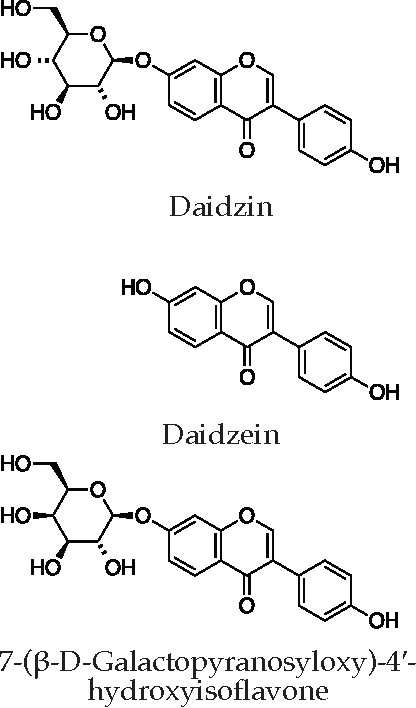
\includegraphics[scale=0.6]{Daidzin2.pdf}
  \vspace{5mm}
  \label{fig:fig1}
\end{marginfigure}




Enzymes catalyze many biological reactions. Often the reaction catalyzed is a desirable synthetic reaction. The stereospecificity and high catalytic efficiency of enzymes makes them prime candidates for use in organic synth\-es\-is. In this exercise we will choose a target reaction, find an enzyme that can catalyze the reaction and then attempt to improve the enzyme by generating mutants. We will focus on the enzyme kinetics of the enzyme candidates with an assay reaction and explore the use of computational tools to deal with large amounts of data.

\section{A Desirable Reaction}

Daidzin is a natural product found in Japanese kudzo vines and soybeen leaves. It is believed to be the active ingredient in herbal medicinal extracts that have been used to treat alcoholism over hundreds of years. Toxic alcohol is removed from the body by the action of \emph{alcohol dehydrogenase}, which cata\-lyz\-es the oxidation of alcohol by NAD\textsuperscript{+} to give acetaldehyde, an even more toxic substance.\sidenote[][0mm]{
``Daidzin: A Potent, Selective Inhibitor of Human Mitochondrial Aldehyde Dehydrogenase.'' W.-M. Keung, B.L. Vallee, \emph{Proc. Natl. Acad. Sci. USA}, \textbf{1993}, \emph{90}, 1247–1251. \url{https://www.jstor.org/stable/2361166}\vspace{2mm}}\textsuperscript{,}\sidenote[][0mm]{``Structure of Daidzin, a Naturally Occurring Anti-Alcohol-Addiction Agent in Complex with Human Mitochondrial Aldehyde Dehydrogenase.'' E.D. Lowe et al., \emph{J. Med. Chem.}, \textbf{2008}, \emph{51}, 4482-4487. \url{https://doi.org/10.1021/jm800488j}\vspace{2mm}}
 Fortunately another enzyme, \emph{aldehyde de\-hy\-drog\-en\-ase}, quick\-ly oxid\-izes the aldehyde to give acetic acid that can be ligated to coenzyme-A and used for energy or, more likely, to make fats. daidzin inhibits \emph{aldehyde de\-hy\-drog\-en\-ase} and this will allow acetaldehyde to build up and make a person very uncomfortable. 

Natural products can be expensive to extract and often the extraction method degrades the material. I have found a cheap source of a related compound, daidzein, from coal tar. This simpler compound is also an inhibitor of \emph{aldehyde de\-hy\-drog\-en\-ase} but it is not soluble in water without the sugar group. I want to glycosylate the daidzein with galactose, rather than the glucose that is present in daidzin. I plan to use an enzyme to catalyze the condensation reaction.

\begin{figure}[h!]

  \caption[0mm]{Condensation of a hemiacetal with a phenol in the synthesis of  7-(\textbeta -D-Galactopyranosyloxy)-4'-hydroxyisoflavone} 
  \vspace{2mm}
    \centering
  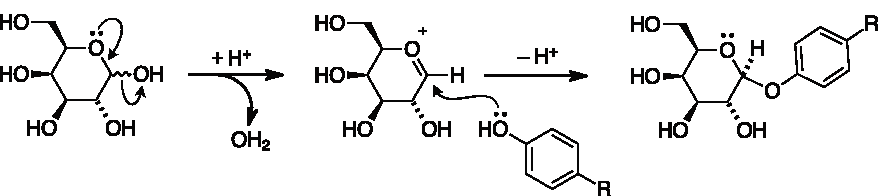
\includegraphics[scale=0.6]{reaction1.pdf}
  \vspace{5mm}
  \label{fig:fig2}
\end{figure}

Using galactose will give us a novel compound that can be patented. Daidzein and galactose are found in foodstuffs and enzymes are a natural material so I plan to simplify the regulatory regime by classifying my molecule as a ``neutraceutical'', a food-based drug that humanity is already experienced with. This will greatly reduce my costs.

\nobibliography{}

\end{document}